\begin{solution}{Question 2}\label{ques:2}
    \begin{question}
    Let $(Setup, H)$ be an SSB-hash. Construct a collapsing hash function (with appropriate domain and co-domain) using the SSB-hash, and prove security of your construction.
    \end{question}
    \tcblower{}
    \begin{proof}
    \begin{claim}
        Let $H_k$ be an SSB-hash with input domain $(\{0,1\}^s)^L$, co-domain $\{0,1\}^l$ with hash key $k$. The same construction of $H_k$ works as a collapsing hash. The property of $H_k$ is that $\prob{\exists x,x' \text{ s.t. } x_i \neq x'_i, H_k(x) = H_k(x')} = negl$ where $x = (x[0], x[1], \ldots x[L-1]), x' = (x'[0], x'[1], \ldots x'[L-1])$
    \end{claim}
    \begin{proof}
        We need to show that if and Adversary can break Collapsing hash, SSB-Hash is broken. SSB-Hash game can be defined as finding a collision $x,x'$. Let us consider the following reduction-
        \begin{figure}[H]
            \centering
            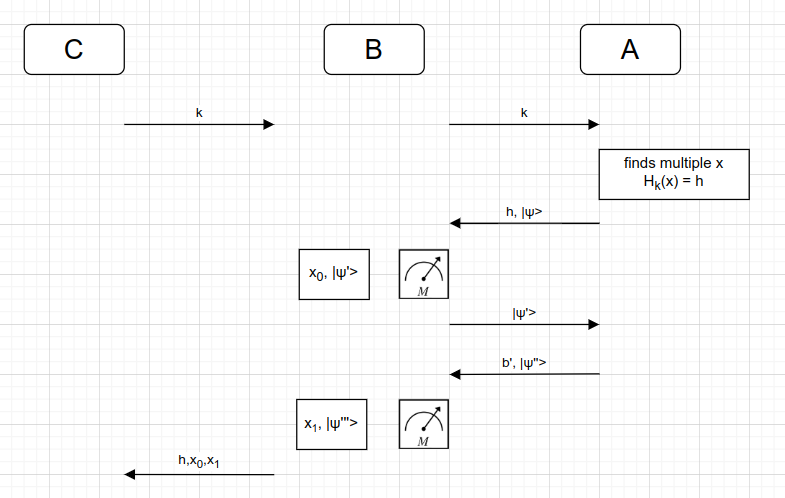
\includegraphics[width = 0.9\textwidth]{image.png}
            \caption{B and C are playing SSB-Hash game, A is playing Collapsing Hash}
            \label{fig:q2}
        \end{figure}
        C gives the key k to B. B forwards it to A and A finds a superposition of $\ket{x} = \ket{\psi}$ such that $H_k(x) = h$ and sends $h, \ket{\psi}$. B measures $\ket{\psi}$ and obtains $\ket{x_0}$ and residual state $\ket{\psi'}$. It sends back $\ket{\psi'}$. A then finds out $b'$ and has a residual state $\ket{\psi''}$ B takes that $\ket{\psi''}$ and measures to obtain $\ket{x_1}$. B then sends $h, \ket{x_0}, \ket{x_1}$ to C.\\
    \end{proof}
    \begin{claim}
        B wins SSB-Hash game with non-negligible probability since $H_k(x_0) = H_k(x_1) = h$ with non-negligible probability.
    \end{claim}
    \begin{proof}
        In the good case, when the A sends a valid superposition $\ket{\psi}$, B measures $\ket{\psi}$ to obtain $\ket{x_0}$ and $H_k(x_0) = h$ with probability 1. When the measured state $\ket{\psi}$ is operated on by A to obtain, it finally has a state $\ket{\psi''}$). This is measured by B to obtain $\ket{x_1}$. Probability of getting a valid $x_1$ such that $H_k(x_1) = h$ is non-negligible (p) (proven in PS4, Q2.1). This is true only if it is not a collapsing hash. Hence:
        \[\prob {\text{finding a collision}} = \prob{H_k(x_0) = h}\times \prob{H_k(x_1) = h} = p\]
        which is non-negligible.
    \end{proof}

    Hence our proposed use of SSB-Hash as a collapsing hash is valid.
    
    
    \end{proof}
\end{solution}
 